\section{Introduction}
Cloud computing was introduced a decade ago with the promise of infinite computing resources available on demand \cite{Armbrust09abovethe}. This model proved to be effective for scaling up search engines\cite{7073834}, social networks\cite{6596496}, and content service providers\cite{6915771} to billions of users around the world. The success can be attributed to several factors: 1) it provides an on-demand pay-as-you-go service to the users which lowers the ownership cost; 2) it provides elasticity of computing, storage, and networking resources which is flexible and scalable; and 3) it facilitates big-data analytics using machine learning technologies due to the highly centralized collocation of intensive computation. However, This centralized model is being challenged by the beginning of a new of computing technology i.e. Internet of Things (IoT).

The Internet of Things (IoT) fosters the connection of massive numbers of objects, sensors, and devices to the network. As per Cisco systems~\cite{ciscoGlance}, 500 billion devices are expected to be connected to the Internet by 2030, and nearly half of the worldwide data will come from sensors~\cite{McAuley}. As the data velocity and volume increases due to the large number of devices that will be connected to the internet, moving the data from IoT devices to the cloud might not be efficient, or might be even infeasible in some cases due to bandwidth constraints~\cite{8289317}. On the other hand, as time-sensitive and location-aware applications emerge~\cite{7389122}, the cloud will not be able to satisfy the low latency, provide location-aware services, or scale to the magnitude of the data that these applications require. Moreover, in some applications, sending the data to the cloud may not be a feasible solution due to privacy concerns~\cite{7849185}. For example, Toyota estimates that the amount of data flowing between vehicles and servers will reach 10 exabytes per month by 2025~\cite{Toyota}. Another example is commercial jets which generate 10 TB of data for every 30 minutes of flight, making it not practical to transport all the data from the edge to the cloud~\cite{ciscoJet}. 

Edge computing is one of the promising solutions for handling the big data that is being produced by the IoT, based on the ability to execute computations and process data at the edge of the network, closer from where the data is being produced. Edge computing suggests the use of smaller servers or single board computers that would have widely distribute processing power in order to speed its results to client devices with improved delays. In this context, edge middleware platforms were created to ease the IoT application development by providing the necessary tools. An edge middleware is defined as a software that serves as an interface between the cloud and the IoT devices, making communication possible among elements that would not otherwise be capable. 

The realization of edge-based middleware platforms suffers from several conceptual and technical limitations. We believe that the seamless integration of edge and cloud systems is one of the main challenges that prevent the efficient utilization of IoT. This requires the developers to manage the platform as a unified set of resources to orchestrate computations, manage devices, and deliver data to users. In addition, there have been a lot of researches towards building edge-based middleware addressing device discovery and management, scalability, managing large data volumes, and privacy and security aspects of the said IoT environment. Therefore there is a strong need to understand the current state-of-the-art for integrated systems that supports fluid management of edge and cloud resources and see if any gaps exist.

%Several surveys on IoT middlewares have been published such as~\cite{7322178, 7582463, Teixeira:2011}. To the best of our knowledge, these surveys only consider a fraction of the currently available IoT middlewares and none of them suggest an architecture that edge middlewares should follow. The contributions of this survey are as follows. First, we present a reference edge middleware architecture, that every existing edge-based middleware solution should follow. Second, we define a set of design goals for each of the layer of the edge middleware architecture and use it for comparing and contrasting the state of the art. And finally based on this we review and present existing issues and gaps, and future research opportunities. 

%The rest of this survey is organized as follows. The motivating use cases for an integration of edge and cloud resources are presented in Section~\ref{sec:usecases}. Section~\ref{sec:arch} presents a reference architecture for enabling end-to-end services in Edge Computing. We propose four architectural layers, along with individual design goals for each of the layers.  Section IV compares platforms and research projects according to the previously described reference architecture. Section~\ref{sec:Challenges} deals with challenges and future work for the realization of edge computing platforms. Section~\ref{sec:Conclusion} summarizes and concludes this survey.

\begin{figure}[hbt!]
    \centering
    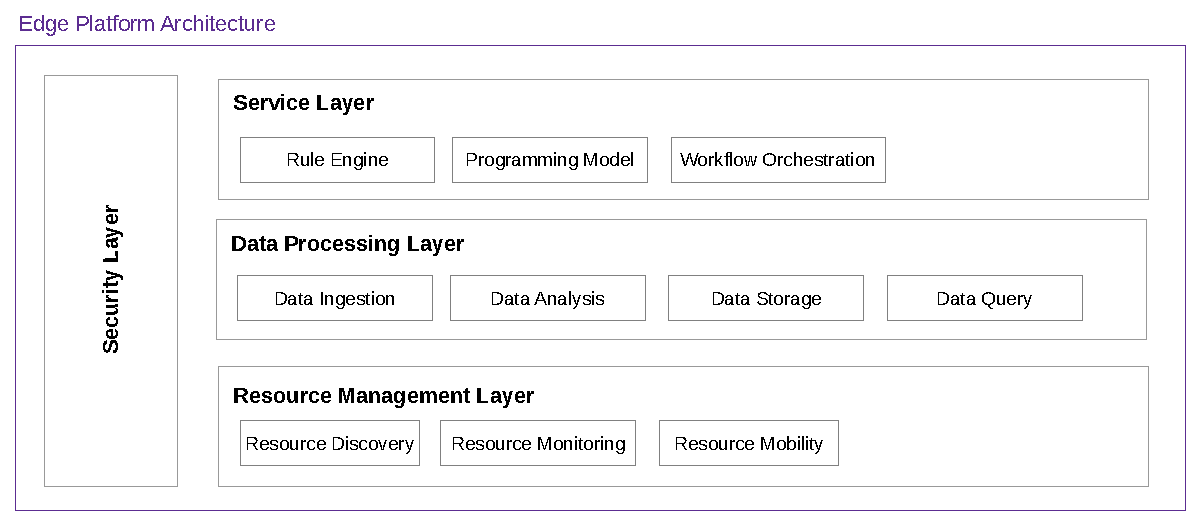
\includegraphics[scale=0.7]{Figures/IoTArchW.pdf}
    \caption{Edge-based middleware reference architecture consisting of four layers, each of them with their respective components.}
    \label{fig:EdgeArch}
\end{figure}

\section{Edge-based Middleware Architecture}\label{sec:arch}

Extensive research and development have been put into creating edge-based middleware systems, there are currently more than 100 edge-based middleware platforms in the market today and the number is continuously growing~\cite{List}. However, not every platform is designed with the same capabilities or architecture. Despite the diversity and large number of edge-based middleware systems, two common architectures emerge:

The majority of IoT platform's architecture follows the cloud-centric approach. They are built on the premise that ingestion, management, and processing of IoT data can be done in the cloud, without any edge computing capabilities. Some examples are: Particle Cloud~\cite{Particle}, Salesforce IoT Cloud~\cite{Salesforce_IoT_Cloud} and If This Then That~\cite{IFTTT}.

The other approach is the end-to-end architecture or middleware centric architecture built on the premise that edge-processing can save huge costs to clients. An Internet of Things (IoT) gateway or middleware is a physical device that serves as the connection point between the cloud and sensors and intelligent devices. All data moving to the cloud, or vice versa, goes through the gateway, which is deployed on single board computers (e.g., Raspberry Pi's), minicomputers, or smart devices (e.g., smartphones, TVs, or refrigerators) to provide management, connectivity, and data pre-processing for sensors.

In this survey, we are only going to focus on the end-to-end or middleware centric architecture. In order to compare and contrast all the existing state of the art, we propose a four-layer edge-based middleware framework that each of the middlewares should consist of. Figure~\ref{fig:EdgeArch} presents the layers and components that need to be included in an edge computing solution. The architecture proposed covers all the requirements that the IoT applications. The edge-based middleware architecture consists of the following four layers: (1) resource management layer, (2) data processing layer, (3) service layer and (4) security layer. Tables ~\cref{tab:full_system_no_goals,tab:full_system_1,tab:full_system_2,tab:full_system_3} summarize the comparison of the available edge-based middleware systems in the market. 

\begin{table}[hbt!]
\caption{Design goals of the resource management layer components of the cited papers in this survey.}
\label{tab:resource}
\resizebox{\textwidth}{!}{%
\begin{tabular}{c|c|c|c|c|c|c|}
\cline{2-7}
                                          & \multicolumn{2}{c|}{Resource Discovery}               & \multicolumn{2}{c|}{Resource Monitoring}              & \multicolumn{2}{c|}{Resource Mobility}                \\ \hline
\multicolumn{1}{|c|}{Paper}               & Distributed               & \begin{tabular}[c]{@{}c@{}}Low \\Overhead\end{tabular}             & Distributed               & \begin{tabular}[c]{@{}c@{}}Low \\ Overhead\end{tabular}              & Distributed               & \begin{tabular}[c]{@{}c@{}}Low \\ Overhead\end{tabular}              \\ \hline
\multicolumn{1}{|c|}{Paganelli et al.~\cite{article}}    & \checkmark & \checkmark &                           &                           &                           &                           \\ \hline
\multicolumn{1}{|c|}{Liu et al.~\cite{6680268}}          & \checkmark &                           &                           &                           &                           &                           \\ \hline
\multicolumn{1}{|c|}{Cirani et al.~\cite{6899579}}       & \checkmark & \checkmark &                           &                           &                           &                           \\ \hline
\multicolumn{1}{|c|}{Jara et al.~\cite{6550579}}         &                           & \checkmark &                           &                           &                           &                           \\ \hline
\multicolumn{1}{|c|}{Zhou et al.~\cite{6664533}}         &                           & \checkmark &                           &                           &                           &                           \\ \hline
\multicolumn{1}{|c|}{Tanganelli et al.~\cite{8086146}}   &                           &                           & \checkmark & \checkmark &                           &                           \\ \hline
\multicolumn{1}{|c|}{M{\"a}enp{\"a}{\"a} et al.~\cite{Maenpaa2012}}      &                           &                           & \checkmark & \checkmark &                           &                           \\ \hline
\multicolumn{1}{|c|}{SEGUE~\cite{SEGUE}}               &                           &                           &                           &                           & \checkmark & \checkmark \\ \hline
\multicolumn{1}{|c|}{Chaufournier et al.~\cite{Chaufournier:2017}} &                           &                           &                           &                           & \checkmark & \checkmark \\ \hline
\multicolumn{1}{|c|}{Farris et al.~\cite{Farris:2017}}        &                           &                           &                           &                           & \checkmark & \checkmark \\ \hline
\end{tabular}
}
\end{table}

\subsection{Resource Management Layer}
The resource management layer is responsible for discovering, identifying, and allocating the available resources for maximum resource utilization in terms of storage, processing, bandwidth, and energy usage. The challenge of the resource management layer is how to manage these limited and geo-distributed resources efficiently. The resource management layer consists of the following components: resource discovery, resource monitoring, and resource mobility. Table~\ref{tab:resource} summarizes the design goals of each of the works focused on the resource management layer.
%to discover, estimate, allocate and monitor resources are the fundamental activities of this layer.

\subsubsection{Design Goals}

The following are the design goals that need to be taken into consideration when developing any of the components of the resource management layer.
\\\\
\textbf{Low Overhead:} The algorithms and protocols of the resource management layer need to offer low runtime overhead when deployed in performance-limited hardware platforms.
\\\\
\textbf{Distributed:} The resource management components also need to be designed in a distributed fashion in order to scale with the number of applications running in the system and with the number of IoT and edge devices.

%\\\\
%\textbf{Dynamic:} The resource management layer should also be capable to make proactive decisions, dynamic deployment, and intelligent decisions based on the understanding of the context of the environments, users and applications requirements.



\subsubsection{Resource Discovery}
The resource discovery component is responsible for efficiently identifying and discovering the geo-distributed IoT sensors. 
The following are some of the work focused only on the resource discovery component. 

Paganelli et al.~\cite{article}propose a system for distributed discovery service. The philosophy behind such system is a peer-to-peer (P2P) approach that adopts the distributed hash table (DHT) techniques, supporting multi-attribute and range queries. Paganelli et al meet both design goals since they use distributed architecture to support the number of growing devices and offers a low overhead algorithm.

Liu et al.~\cite{6680268} propose a distributed resource discovery architecture (DRD) for M2M applications. The DRD supports
heterogeneous devices in resource description registration and discovery of resource value. It achieves interoperability among
heterogeneous devices in disparate networks and enables resource access from the Internet. In the DRD, a resource registration component is designed for storing resource descriptions; a resource discovery component is designed to retrieve resource values on behalf of clients after getting address information by looking up resource descriptions. The DRD utilizes a peer-to-peer overlay to distribute workload and avoids a single point of failure. Liu et al. resource discovery mechanism only meet the distributed goal since the system is build using a peer-to-peer architecture to efficiently discover the resources in a decentralized manner. It does not meet the low overhead since it used HTTP to communicate and discover resources~\cite{8088251}. The reason being that HTTP runs on TCP, therefore it incurs all TCP connection overheads for connection establishment and closing.

Cirani et al.~\cite{6899579} presents a scalable and self-configurable P2P architecture for service discovery (SD). Utilization of
P2P technologies enables deployment of distributed and large scale infrastructure for SD. IoT gateway acts as a backbone of the SD architecture. The gateway keeps track of any things joining or leaving its network and updates the list maintained at its CoAP server. Cirani et al. resource discovery mechanism satisfies both goals since it used a distributed P2P architecture for discovering resources and it used CoAP a lightweight messaging system that uses UDP~\cite{8088251} for keeping track of all the resources.

Jara et al.~\cite{6550579} presents a centralized mechanism for discovering devices based on context-awareness and geo-location. An infrastructure called 'digcovery' for maximizing efficiency and sustainability of deployments offering the framework to allow users to register/include their own sensors into a common infrastructure, and access/discover the available resources through a mobile phone. Jara et al. only satisfy the low overhead goal of the resource discovery mechanism since it uses a centralized architecture for discovering devices. It is well known that centralized architecture suffers from single point-of-failure and scalability when the number of IoT devices grows. 

Zhou et al.~\cite{6664533} present an ontology focused web service matching algorithm aimed at IoT systems. As a proof-of-concept, they have portrayed an ontology concept for the vehicular sensor. The algorithm reference semantic similarity and semantic relativity calculation method used in text retrieval. Zhou et al. only satisfy the low overhead goal since resource discovery mechanism claims that the algorithm has good scalability, and it can be applied to different fields only need to replace the domain ontology.

\subsubsection{Resource Monitoring}
The resource monitoring component is responsible for controlling and managing hardware and software infrastructures. It also provides information and performance indicators for both platforms and applications to assist in the decision of allocating the resources. It also monitors the state of the resources in the event of failure. The following are some of the work focused only on the resource monitoring component.

Tanganelli et al.~\cite{8086146} propose an approach that leverages the CoRE Resource Directory interface and the CoAP protocol to expose a standard interface for global discovery and access. Where the IoT gateways are federated through a P2P overlay implemented by a Distributed Hash Table (DHT), which is exploited to share the information on IoT resources available across multiple domains. This approach is able to satisfy both design goals since it is distributed and achieves low overhead on constrained devices.

M{\"a}enp{\"a}{\"a} et al.~\cite{Maenpaa2012} propose an architecture for wide area sensor and actuator networking. The architecture is based on combining two protocols being standardized by the Internet Engineering Task Force, REsource LOcation And Discovery (RELOAD) and Constrained Application Protocol (CoAP). The architecture also enables a peer-to-peer federation of geographically distributed Wireless Sensor Networks (WSNs). Just like the previous approach this approach also satisfies both design goals.

\subsubsection{Resource Mobility}
The resource mobility component is responsible for moving computations between edge nodes, in order to achieve the requirements of the IoT applications. The following are some of the work focused only on the resource mobility component.

SEGUE~\cite{SEGUE} study the service migration problem in edge clouds, in response to user movement and network performance. The solution is based on Markov Decision Process (MDP) that considers network state and server response time in making migration decisions. SEGUE meets all the design goals since it was carefully evaluated to showcase the real-time performance, scalability, and dynamicity by using real mobility trace of 320 taxis in Rome. 

Chaufournier et al.~\cite{Chaufournier:2017}, suggested to use multi-path TCP for live migration of VMs across edge nodes to improve VM migration time and network transparency of applications.  Chaufournier et al. resource mobility approach also achieves all the goals since it proposed the uses of multi-path TCP and claims that increases the migration throughput by 6x and reduces the time by 50\% in some cases.

Farris et al.~\cite{Farris:2017}, define two integer linear programming (ILP) optimization schemes to minimize QoE degradation and cost of replica deployment in service replication for MEC. Farris et al. resource mobility also meets all the goals since it was designed to cope with the limitation of resource-constrained edge nodes and showcased the scalability in terms of users and the dynamicity of the algorithm.

\begin{table}[h!]
\caption{Design goals of the data processing layer components of the cited papers in this survey.}
\label{tab:processing}
\begin{tabular}{c|c|c|c|c|c|c|c|c|c|c|c|c|}
\cline{2-13}
                                   & \multicolumn{3}{c|}{Data Ingestion}                                 & \multicolumn{3}{c|}{Data Analysis}                                                & \multicolumn{3}{c|}{Data Storage}                                                 & \multicolumn{3}{c|}{Data Query}                                                   \\ \hline
\multicolumn{1}{|c|}{Project}        & \rotatebox[origin=c]{90}{Real-Time} & \rotatebox[origin=c]{90}{Distributed}               & \rotatebox[origin=c]{90}{Scalable}                  & \rotatebox[origin=c]{90}{Real-Time}                 & \rotatebox[origin=c]{90}{Distributed}               & \rotatebox[origin=c]{90}{Scalable}                  & \rotatebox[origin=c]{90}{Real-Time}                 & \rotatebox[origin=c]{90}{Distributed}               & \rotatebox[origin=c]{90}{Scalable}                  & \rotatebox[origin=c]{90}{Real-Time}                 & \rotatebox[origin=c]{90}{Distributed}               & \rotatebox[origin=c]{90}{Scalable}                  \\ \hline
\multicolumn{1}{|c|}{Apache Kafka~\cite{kafka}} &             & \checkmark & \checkmark &                           &                           &                           &                           &                           &                           &                           &                           &                           \\ \hline
\multicolumn{1}{|c|}{Mosquitto~\cite{mosquitto}}    &             & \checkmark & \checkmark &                           &                           &                           &                           &                           &                           &                           &                           &                           \\ \hline
\multicolumn{1}{|c|}{RabbitMQ~\cite{RabbitMQ}}     &             & \checkmark &                           &                           &                           &                           &                           &                           &                           &                           &                           &                           \\ \hline
\multicolumn{1}{|c|}{ActiveMQ~\cite{HiveMQ}}     &             & \checkmark &                           &                           &                           &                           &                           &                           &                           &                           &                           &                           \\ \hline
\multicolumn{1}{|c|}{Heron~\cite{heron}}        &             &                           &                           &                           & \checkmark & \checkmark &                           &                           &                           &                           &                           &                           \\ \hline
\multicolumn{1}{|c|}{Storm~\cite{storm}}        &             &                           &                           &                           & \checkmark & \checkmark &                           &                           &                           &                           &                           &                           \\ \hline
\multicolumn{1}{|c|}{Flink~\cite{flink}}        &             &                           &                           &                           & \checkmark & \checkmark &                           &                           &                           &                           &                           &                           \\ \hline
\multicolumn{1}{|c|}{MillWheel~\cite{millwheel}}    &             &                           &                           &                           & \checkmark & \checkmark &                           &                           &                           &                           &                           &                           \\ \hline
\multicolumn{1}{|c|}{Spark~\cite{spark}}        &             &                           &                           &                           & \checkmark & \checkmark &                           &                           &                           &                           &                           &                           \\ \hline
\multicolumn{1}{|c|}{ApacheEdgent~\cite{edgent}} &             &                           &                           & \checkmark & \checkmark & \checkmark &                           &                           &                           &                           &                           &                           \\ \hline
\multicolumn{1}{|c|}{LMC~\cite{8102173}}          &             &                           &                           & \checkmark &                           & \checkmark &                           &                           &                           &                           &                           &                           \\ \hline
\multicolumn{1}{|c|}{DataFlog~\cite{DataFog:2018}}     &             &                           &                           &                           &                           &                           & \checkmark & \checkmark & \checkmark & \checkmark & \checkmark & \checkmark \\ \hline
\multicolumn{1}{|c|}{FogStore~\cite{Gupta:2018, Mayer2017FogStore}}     &             &                           &                           &                           &                           &                           & \checkmark & \checkmark & \checkmark & \checkmark & \checkmark & \checkmark \\ \hline
\multicolumn{1}{|c|}{Moon et. al.~\cite{8190803}} &             &                           &                           &                           &                           &                           &                           &                           &                           &                           & \checkmark & \checkmark \\ \hline
\multicolumn{1}{|c|}{IOTMDB~\cite{6468294}}       &             &                           &                           &                           &                           &                           &                           &                           &                           &                           & \checkmark & \checkmark \\ \hline
\end{tabular}
\end{table}

\subsection{Data Processing Layer}

The data processing layer is responsible for consolidating data from multiple sources, processing the data, and making them available. State-of-the-art data processing layers are known to be data-intensive tasks, due to the constant reading and writing from an to disk resulting in the inability to performing real-time data analytics when deployed on edge constrained devices. The data processing layer consists of the following components: data ingestion, data analysis, data storage, and data query. Table~\ref{tab:processing} summarizes the design goals of each of the works focused on the data processing layer.

\subsubsection{Design Goals}

The following are the design goals that need to be taken into consideration when designing any of the components of the data processing layer.
\\\\
\textbf{Distributed:} The data processing components should support distributed information processing, distributed computing capabilities, distributed storage and query. In order to address the variable number of devices, services, and users at any given point in time.
\\\\
\textbf{Scalable:} The scalable term refers to the ability of the data processing component to handle a growing number of
clients. The data processing components also need to be scalable also to address the needs of a variable number of devices, services, and users. 
\\\\
\textbf{Real-Time:} The real-time term refers to the ability to achieve low processing latency as the number of messages increases. The data processing components need to be able to process data in real-time either in edge constrained devices such as Raspberry Pis or smartphones and the cloud. Since IoT applications are latency sensitive as we described in section~\ref{sec:usecases}. 

\subsubsection{Data Ingestion}

The data ingestion component gathers data from multiple sources and brings them to the pipeline for processing. The following are some of the work focused only on the data ingestion component.

Apache Kafka~\cite{kafka} is one of the most popular frameworks available, it is an open source framework used for building real-time data pipelines and streaming apps. It is horizontally scalable, fault-tolerant, and runs in production in thousands of companies. Apache Kafka meets three of the four design goals, the reason Apache Kafka does not offer real-time processing at the edge of the network, because it was not designed to be deployed in constrained devices, it was designed to be deployed at the cloud. 

Mosquitto~\cite{mosquitto} is an open source message broker that implements the MQTT protocol. It provides a lightweight method of carrying out messaging using a publish/subscribe model. This makes it suitable for Internet of Things messaging such as with low power sensors or mobile devices such as phones, embedded computers or microcontrollers. Even though Mosquitto was created for the need to achieve real-time message handling, Scalagent published a survey where they stress test the Mosquitto and show that it can succeed at handling 60.000 publishers but it requires high transmission latency and high CPU usage~\cite{mqtt}.

RabbitMQ~\cite{RabbitMQ} is lightweight and easy to deploy on-premises and in the cloud. It supports multiple messaging protocols. RabbitMQ can be deployed in distributed and federated configurations to meet high-scale, high-availability requirements. Similarly to Mosquitto, RabbitMQ in the scaleagent tests shows that it can only handle 8000 publishers producing 8000 messages per second. Not being able to achieve real-time analytics~\cite{mqtt}.

ActiveMQ~\cite{HiveMQ} is the most popular open source, multi-protocol, Java-based messaging server. It supports industry-standard protocols so users get the benefits of client choices across a broad range of languages and platforms. ActiveMQ also suffers from the same problems as Mosquitto and RabbitMQ, has high message transmission latency and cannot handle more than 20.000 publishers~\cite{mqtt}.

\subsubsection{Data Analysis}

The data analysis is a process of inspecting, cleansing, transforming, and modeling data with the goal of discovering useful information and decision-making. The following are some of the work focused only on the data analysis component.

Heron~\cite{heron} is a real-time analytics platform developed by Twitter, it's designed for speedy performance, low latency, isolation, and reliability. Heron meets all the design goals except for the real-time data analytics at the edge. Because it was designed to be deployed in large clusters at the core of the network.

Storm~\cite{storm} is an open source distributed real-time computation system. Storm makes it easy to reliably process unbounded streams of data in real-time. Similarly, Storm was also designed to be deployed in the cloud.

Flink~\cite{flink}  is a framework and distributed processing engine for stateful computations over unbounded and bounded data streams. Flink has been designed to run in all common cluster environments, perform computations at in-memory speed and at any scale. Flink was also designed for the cloud and not for the edge.

MillWheel~\cite{millwheel} is a framework for building low-latency data-processing applications that are widely used at Google. Users specify a directed computation graph and application code for individual nodes, and the system manages persistent state and the continuous flow of records, all within the envelope of the framework's fault-tolerance guarantees. MillWheel just like Heron, Storm, and Flink was designed to be deployed in large clusters.

Spark~\cite{spark} is an open-source distributed general-purpose cluster computing framework with an in-memory data processing engine that can do analytics, machine learning and graph processing on large volumes of data at rest or in motion.

Apache Edgent~\cite{edgent} is a programming model and micro-kernel style runtime that can be embedded in gateways and small footprint edge devices enabling local, real-time, analytics on the continuous streams of data coming from equipment, vehicles, systems, appliances, devices, and sensors of all kinds (for example, Raspberry Pis or smartphones). Apache Edgent is the only stream processing engine that was designed to be deployed on edge devices, allowing it to achieve all the design goals.

LMC~\cite{8102173} a framework that aims at enabling cross-platform code execution on constrained IoT devices. LCM meets the real-time and the scalable design goals since it was designed to constrained devices, but it doesn't meet the distributed since there is no current support.

\subsubsection{Data Storage}

Due to the ever-increasing deployment of bandwidth-intensive IoT platforms (especially cameras), there is an increasing pressure on the bandwidth to transport data back and forth between the edge and the Cloud. This factor point to the need for a more efficient management of the data and the computation on the data at the edge of the network. Building a storage system on an edge computing infrastructure has its own set of peculiar challenges. The wide geo-distribution, heterogeneous and the constrained nature of this
infrastructure requires data-partitioning and replication policies that are commensurate with the latency requirements of the applications. The following are some of the work focused only on the data storage component.

DataFlog~\cite{DataFog:2018} is a distributed indexing mechanism that performs data placement (both among edge nodes, and between the edge and the Cloud) based on spatiotemporal attributes to support efficient queries involving multiple edge nodes. DataFlog is able to achieve all the design goals for the data storage layer since it uses distributed indexing mechanism, it supports efficient queries and it can scale since it uses a P2P network and can be deployed in any environment.

FogStore~\cite{Gupta:2018}~\cite{Mayer2017FogStore} is a key-value store for event-based systems, that exploits the concept of relevance to guarantee low-latency access to relevant data with strong consistency guarantees while providing tolerance from geographically correlated failures. FogStore was designed by the same authors of DataFog and it also meets all the design goals, just like DataFlog.

\subsubsection{Data Query}

Similarly to the data storage, once data has been stored it needs to be accessed as well. The following are some of the research work on creating edge query systems. The following are some of the work focused only on the data query component.
 
Moon et al.~\cite{8190803} propose a data management and searching system based on blockchain which ensures security by using ECDSA digital signature and SHA-256 hash function. Moon et al. are able to meet all the goals for the data query layer except for the real-time since they are using heavy blockchain algorithms.

IOTMDB~\cite{6468294} is an Internet of Things storage management architecture based on NoSQL to meet the needs of IoT data storage. IOTMDB concerns about how to reasonably and effectively store massive IoT data, but also cares for data sharing and collaboration. IOTMDB is able to satisfy all the design goals except for the real-time, the results presented in the paper are big.

\begin{table}[h!]
\caption{Design goals of the service layer components of the cited papers in this survey.}
\label{tab:service}
\resizebox{\textwidth}{!}{%
\begin{tabular}{c|c|c|c|c|c|c|c|}
\cline{2-8}
                                       & \multicolumn{2}{c|}{Rule Engine}                      & \multicolumn{2}{c|}{Programming Model}                & \multicolumn{3}{c|}{Workflow Orchestrator}                                        \\ \hline
\multicolumn{1}{|c|}{Paper}            & Scalable                  & \begin{tabular}[c]{@{}c@{}}Low \\ Overhead\end{tabular}              & Expressive                 & Extensible                  & Dynamic                   & Scalable                  & \begin{tabular}[c]{@{}c@{}}Low \\ Overhead\end{tabular}              \\ \hline
\multicolumn{1}{|c|}{Chui et. al.~\cite{5277977}}     & \checkmark & \checkmark &                           &                           &                           &                           &                           \\ \hline
\multicolumn{1}{|c|}{Lica et. al.~\cite{7314063}}     &        \checkmark                   &                           &                           &                           &                           &                           &                           \\ \hline
\multicolumn{1}{|c|}{Mobile-Fog~\cite{Hong:2013}}       &                           &                           & \checkmark & \checkmark &                           &                           &                           \\ \hline
\multicolumn{1}{|c|}{Rabel~\cite{ravel-riliskis-iotapp15}}            &                           &                           &        \checkmark                   & \checkmark &                           &                           &                           \\ \hline
\multicolumn{1}{|c|}{Fabryq~\cite{Etemadi2014FabryqUP}}           &                           &                           &       \checkmark                     &          \checkmark                  &                           &                           &                           \\ \hline
\multicolumn{1}{|c|}{FogFlow~\cite{8022859}}          &                           &                           & \checkmark & \checkmark &                           &                           &                           \\ \hline
\multicolumn{1}{|c|}{Eidenbenz et al.~\cite{Eidenbenz:2016}} &                           &                           &                           &                           &                           &                           & \checkmark \\ \hline
\multicolumn{1}{|c|}{Taneja et al.~\cite{Taneja:2017}}    &                           &                           &                           &                           &                           & \checkmark & \checkmark \\ \hline
\multicolumn{1}{|c|}{DROPLET~\cite{8457776}}          &                           &                           &                           &                           & \checkmark & \checkmark & \checkmark \\ \hline
\multicolumn{1}{|c|}{Ghosh et al.~\cite{Ghosh:2018}}     &                           &                           &                           &                           & \checkmark &                           &                           \\ \hline
\end{tabular}
}
\end{table}

\subsection{Service Layer}
The Service Layer defines an application's set of available operations from the perspective of interfacing client layers. It encapsulates the application's business logic, controlling transactions and coordinating responses in the implementation of its operations. The service layer consists of the following components: rule engine, programming model, and workflow orchestrator. Table~\ref{tab:service} summarizes the design goals of each of the works focused on the service layer.

\subsubsection{Design Goals}

The following are the design goals that need to be taken into consideration when creating any of the components of the service layer.
\\\\
\textbf{Low Overhead} The service layer components need to be able to process data in real-time, i.e. providing fast analysis and data queries when deployed in performance-limited hardware platforms.
\\\\
\textbf{Scalable} The service layer components need to offer good scalability, since there is going to be a large number of rules and a large number of operators that need to be placed.
\\\\
\textbf{Dynamic} This design goal only applies to the workflow orchestrator. The workflow ochestrator needs to be able to orchestrate the workflows based on the runtime characteristics of the nodes. 
\\\\
\textbf{Expressive} This design goal only applies to the programming model. The programming model needs to be easy to express ideas, algorithms, tasks in an easy-to-read and succinct way.
\\\\
\textbf{Extensible} This design goal also only applies to the programming model. The programming model needs to flexible enough that if new capabilities are needed, they can be added to the software without major changes to the underlying architecture.

%\textbf{Portability} The service layer components should be able to be deployed in any cloud or edge enviroment. 
%The recent trend of emergence of heterogeneous subsystems in smart home environment often leads to interoperability problem in managing such systems. Interoperability is defined as the ability of two or more entities to exchange information and to use the information that has been exchanged [2]. In smart home environment, interoperability is concerned with message exchange between two or more subsystems and performing interoperation in a federated and satisfactory manner without the need for external intervention. 

\subsubsection{Rule Engine}

The Rule Engine makes it possible to build IoT applications that gather, process, analyze and act on data generated by connected devices at a global scale without having to manage any infrastructure. A rule engine applies a set of rules and facts to deduce conclusions, searching the rules until it finds one where the IF clause is known to be true. The following are some of the work focused only on the rule engine component.

Chui et al.~\cite{5277977} propose a rule-based framework for the management of heterogeneous systems in a smart home environment. The proposed framework is based on an ECA rule mechanism with SOAP technology that provides interoperability among sensors and actuators systems. Chui et al rule engine satisfies all the design goals since they use an Event-Condition-Action (ECA) pattern which allows them to scale the system as the number of rules grows and achieve low overhead. 

Lica et. al~\cite{7314063} proposed a rule-based semantic architecture with the aim to help common end-users in defining their building automation applications. This architecture addresses the main issues involved in application management in an Internet of Things context, such as: (i) application and context modeling, by means of ECA Rule, System, High-Level States and High-Level Actions abstractions, (ii) application creation and control, through the introduction of a visual IDE, (iii) execution environment definition, by means of a Semantic Framework and an Action Engine, (iv) physical device management, by introducing a low-level layer that abstracts device heterogeneity. Lica et. al approach only satisfies the scalability goal since its an initial approach and they specify that further development needs to be carried out.

\subsubsection{Programming Models}
Due to the high dynamicity of edge resource, heterogeneity of cloud and edge resources deploying low latency and scalable applications can be tricky. For this reason, there is a need for high-level programming models that simplify the development of IoT applications across the edge and the cloud. The following are some of the work focused only on the programming model component.

Mobile-Fog~\cite{Hong:2013} is a high-level programming model for future Internet applications that are geospatially distributed, large-scale, and latency-sensitive. Mobile-Fog only Rabel satisfies both design goals since it uses a high-level API to program the sensors, making it easy to learn.

Rabel~\cite{ravel-riliskis-iotapp15} proposes a novel approach for programming applications across 3-tiers using a distributed extension of the Model-View-Controller architecture. Ravel introduces the concept of space, which binds particular models, controllers, and views to a specific device. The networking complexities between devices are hidden by the distributed model that automatically synchronizes whenever possible. Rabel satisfies both design goals since it uses a high-level API.

%Wenger et al.~\cite{7809704} a programming language and system for a three-layered Cloud of Things (CoT) system. Presents a design of a polyglot language for CoT that combines two existing languages C and JavaScript and runs on the distributed virtual machine. Satisfies both goals since the programming language is C, a well-known programming language.

%WuKong et al.~\cite{Reijers2013DesignOA, Reijers2011BuildingIM} use a flow-based programming paradigm in a familiar Java environment. The developer constructs an application from logical components in WuKong's library and later distributes the application as a binary executable for embedded Java VM.

%Exemplar~\cite{Hartmann:2007} allows the developer to demonstrate the desired physical interaction and bind it to a resulting action. The system analyzes the sensor traces and classifies different interactions (tilting a head left or right). 

Fabryq et al.~\cite{Etemadi2014FabryqUP} allow developers to write an embedded-gateway-cloud application as a centralized Javascript application that interacts with the cloud and embedded device through RPC function calls. These and many other techniques allow a developer to explore quickly and prototype an MGC application. Fabryq et al approach also satisfies both design goals since it uses Javascript as the main programming language and also has a high-level API to program the sensors, making it easy to learn.

FogFlow~\cite{8022859} extends the dataflow programming model with declarative hints based on the widely used standard NGSI, which leads to two benefits for service developers: 1) fast and easy development of fog computing applications, this is because the proposed hints hide lots of task configuration and deployment complexity from service developers; 2) good openness and interoperability for information sharing and data source integration, this is because NGSI is a standardized open data model and API and it has been widely adopted by more than 30 cities all over the world. FogFlow satisfies both design goals since it extends the cloud-based dataflow programming model with standard-based APIs and makes it suitable for the cloud-edge environment, making it easy to learn. FogFlow also satisfies both design goals since it uses Javascript or Python as a programming language and has a high-level API, making it easy to learn.

\subsubsection{Workflow Orchestrator}

The Workflow Orchestrator consists of defining how to accommodate the application components (i.e., operators) on the available resources of the network topology to optimize one or more performance metrics. A key challenge is to automatically decide how to partition such operations among edge and cloud compute resources, in order to minimize the overall completion time of the entire graph of operations. The workflow placement has been proved to be at least NP-Hard~\cite{Benoit:2013}. The following are some of the work focused only on the workflow orchestrator component.

Eidenbenz et al.~\cite{Eidenbenz:2016} evaluated Series-Parallel-Decomposable Graphs (SPDG) from its parallelism degree to decompose the application graph and by an approximation algorithm to determine the placement. Eidenbenz et al. only satisfy the real-time design goals since its only a theoretical approach.

Taneja et al.~\cite{Taneja:2017} offer a naive approach deploying the application graph across cloud and edge using a constraint-sensitive approach. Taneja et al meet all the design goals except for the dynamicity, the approach doesn't take into consideration network connectivity or failure of nodes.

%Cardellini et al.~\cite{Cardellini:1002} and Chen \textit{et al.} \cite{Chen:2017} consider the monetary cost. The former approach introduces a model considering monetary price as the cost per unit of data transmitted along the network path between two machines. The latter covers prices for the IoT application placement using VMs, however, they create a uniform pricing model to VMs given that the cost of electricity, infrastructure, personnel, and taxes are similar within the same region. 

DROPLET~\cite{8457776} is a scalable dynamic programming algorithm, to partition operations in IoT applications across shared edge and cloud resources, while minimizing the completion time of the end-to-end operations. DROPLET achieves all the design goals since it is able to react and adapt to dynamic events and is capable of performing real-time decisions and it is able to scale polynomially with increasing the number of operators. 

Ghosh et al.~\cite{Ghosh:2018} propose a Genetic Algorithm (GA) meta-heuristic for distributing analytics across edge and Cloud resources to support IoT applications. The main goal of the genetic algorithm is to minimize the end-to-end latency. Ghosh et al approach only meet one of the design goals since it takes between 1 - 26 seconds for placing 1 - 50 operators, making it not real-time or scalable when the number of operators grows.

\begin{table}[h!]
\begin{adjustwidth}{1.8cm}{3cm}
\caption{Design goals of the security layer components of the cited papers in this survey.}
\label{tab:security}
\begin{tabular}{|c|c|c|}
\hline
Paper            & End-to-End Security       & Data Privacy              \\ \hline
Endler et al.~\cite{8241993}    &                           & \checkmark \\ \hline
Lu. et al.~\cite{7869305}       &                           & \checkmark \\ \hline
Shi et al.~\cite{shi}       &                           & \checkmark \\ \hline
Behrens et al.~\cite{7899405}    & \checkmark &                           \\ \hline
Mukherjee et al.~\cite{7987191} & \checkmark &                           \\ \hline
Kothmayr et al.~\cite{6424088}  & \checkmark &                           \\ \hline
\end{tabular}
\end{adjustwidth}
\end{table}

\subsection{Security Layer}
Internet of Things (IoT) consists of thousands of devices that generate, process, and exchange vast amounts of security and safety-critical data as well as privacy-sensitive information, and hence keeping that information private and secure is a big and important challenge that needs to be taken into consideration. The following are some of the work focused only on the end-to-end security component. Table~\ref{tab:security} summarizes the work focused on the security layer.

\subsubsection{Data privacy}

Since the IoT makes large volumes of information easily available through remote access mechanisms, privacy protection in IoT is challenging. The following are some of the work focused only on the data privacy component.

Endler et al.~\cite{8241993} present ContextNet a middleware which consists of scalable software infrastructure for enabling cloud-based communication with mobile devices (SDDL), and parallel data stream processing facilities in the cloud/cluster. The Scalable Data Distribution Layer (SDDL) is a communication infrastructure that connects mobile nodes to stationary nodes (i.e. the SDDL Core), executing in a cloud or a cluster. The stationary nodes may be application specific servers, gateways for connection with the mobile nodes, or monitoring and control nodes for displaying the mobile nodes current position on maps, managing and communicating with groups of mobiles, and sending message to individual mobile nodes. 

Lu et al.~\cite{7869305} present a lightweight privacy-preserving data aggregation scheme, called Lightweight Privacy-preserving Data Aggregation, for fog computing-enhanced IoT. The proposed LPDA is characterized by employing the homomorphic Paillier encryption, Chinese Remainder Theorem, and one-way hash chain techniques to not only aggregate hybrid IoT devices' data into one, but also early filter injected false data at the network edge. 

Shi et al.~\cite{shi} describes a Private Stream Aggregation (PSA) algorithms which allow users to upload a stream of encrypted data to an untrusted aggregator, and allow the aggregator to decrypt (approximate) aggregate statistics for each time interval with an appropriate capability.

\subsubsection{End-to-End Security}

To preserve user security and privacy it is critical that the communication link among the IoT devices and the remote hosts or servers that are interested in accessing the critical data is secured, in order not to leak personal data. It is very important to understand which protocols are able to provide the right level of security without burdening the limited resources of the constrained edge devices. The limited computational capacity, the low amount of memory, and the constraints on energy consumption make the design of these protocols particularly hard and complicated. 

Behrens et al.~\cite{7899405} present a single end-to-end Application Security Layer (ASL). The ASL caters for reliable and confidential communications within a constrained Internet of Things (IoT) environment. To provide a secure key exchange and to set up a secure data connection, the TLS protocol is used. This paper studies the use of TLS over JSON via a CoAP RESTful service. This method provides a way for end-to-end communication flexibility and potentially retain identity information for repudiation. 

Mukherjee et al.~\cite{7987191} present the design and implementation of a middleware featuring "intermittent" and "flexible" end-to-end security for cloud-fog communications. Intermittent security copes with unreliable network connections, and flexibility is achieved through security configurations that are tailored to application needs.

Kothmayr et al.~\cite{6424088} introduce the first fully implemented two-way authentication security scheme for the Internet of Things (IoT) based on existing Internet standards, especially the Datagram Transport Layer Security (DTLS) protocol. The proposed security scheme is based on the most widely used public key cryptography (RSA) and works on top of standard low power communication stacks. 

\section{Commercial and Academic Edge Middelware Systems}
In this section we analyze the similarities and differences amongst all the currently available edge middleware systems, to do that we use the proposed edge platform architecture and the goals of each of the layers described in the previous section. Tables~\ref{tab:full_system_no_goals},\ref{tab:full_system_1},\ref{tab:full_system_2},\ref{tab:full_system_3} summarize and offer more details on all the edge middelware surveyed systems, including the design goals that each component satisfies.

AWS Greengrass~\cite{greengrass} is a software that lets you run local compute, messaging, data caching, sync, and Machine Learning inference capabilities on connected devices in a secure way. AWS Greengrass consists of all the four layers presented in section~\ref{sec:arch}. The main limitations of AWS Greengrass are the centralized architecture of the resource management layer, the lack of storage and query of the data processing layer,  the use of a similar MQTT broker to Mosquitto for data ingestion violating the real-time design goal for the data processing layer and the lack the workflow orchestration component in the service layer, leaving it to the end user for the management and provisioning of the workflows. 

Azure IoT Edge~\cite{azure} is a comprehensive collection of services and solutions designed to help create end-to-end IoT applications on Azure Cloud. This service is meant for analyzing data at the edge of the network, instead of in the cloud. Azure IoT similarly to AWS they take security very seriously, they use certificate-based authentication as the primary mechanism for authentication for the Azure IoT Edge platform. Azure IoT also implements all four layers proposed in section~\ref{fig:EdgeArch}. Azure IoT only misses two components, the first one is the workflow orchestrator from the service layer and the data privacy at the security layer. Azure IoT uses a similar MQTT broker to Mosquitto making it not able to achieve real-time analytics.

EAaaS~\cite{8029781} a scalable analytic service for enabling real-time edge analytics in IoT scenarios. The main focus of the EAaaS is to propose a unified rule-based analytic model to ease user's programming efforts in specifying rule-based analytic logic. In addition, they put large attention on making the system be as lightweight, scalable, and achieve real-time data analytics at the edge. EAaaS implements two of the four layers, it does not implement the resource management layer or the security layer and misses some components on the layers that implements. The first components missing are from the data processing layer, EAaaS does not allow to store or query data at the edge of the network. From the service layer, EAaS does not implement the workflow orchestrator forcing the end user to decide where to place computations to achieve optimal performance. 

Google Cloud IoT Edge~\cite{google} is a set of fully managed and integrated services that allows to easily and securely connect, manage, and ingest IoT data from globally dispersed devices at a large scale, process and analyze/visualize that data, and implement operational changes and take actions as needed. Google Cloud IoT Edge follows the same path as the AWS Greengrass, implements all four layers but misses some critical components on some of the layers. Google Cloud IoT Edge does not support the ability to store or query at the edge of the network. In addition just like all the commercial systems surveyed so far, it also implements a similar broker to Mosquitto, making it hard to achieve real-time analytics. Google Cloud IoT Edge does not offer the ability to orchestrate application between the edge and the cloud.

Everyware IoT~\cite{everyware} is an integrated platform for the Internet of Things which provides propitiatory IoT gateways for any industry vertical, an open edge framework and a modular cloud infrastructure to connect field devices to business analytics and enterprise applications. Everyware IoT implements all four layers but misses some critical components in all the layers. Similar to AWS, Azure, and Google, lacks the query and storage support at the edge of the network and uses a similar Mosquitto broker for the data ingestion. Additionally, Everyware IoT lacks the rule engine of the service layer making it not possible to trigger or react to events that happen at the edge of the network.

Predix~\cite{predix} is General Electric's commercial software platform for the collection and analyzing data from industrial machines. For Predix security is one of the most important aspects, which supports a wide range of industry, regional, privacy and data governance regulations, and encompass perimeter security, data security, and access control. Predix implements all four layers but misses some critical components. Predix does not offer resource monitoring, storage or query. In addition, it also doesn't offer the ability to orchestrate workflows between the edge and the cloud of the network.

Bosch IoT~\cite{bosch} is a commercial suite that consists of various cloud-enabled services and software packages that enable the fast, easy, and secure development of sustainable applications in the Internet of Things. Using wireless communication, the Bosch IoT Edge Gateway Software connects low-energy, battery-powered sensors. The environmental data from these sensors are remotely captured in the Bosch IoT Cloud. Bosch IoT implements all four layers but misses some components. Bosch IoT does not offer the rule engine or the workflow orchestrator of the service layer, and just like all other commercial systems it also implements a similar broker to Mosquitto. 

Yanzi~\cite{yanzi} is an academic platform that enables IoT solutions that are easy to deploy, manage and visualize. For thousands of sensors. Yanzi implements three of the four layers, lacking the resource management layer and some critical components on other layers. In the service layer, Yanzi misses the rule engine and the workflow orchestrator, and in the security layer, it misses the data privacy component.

R-Pulsar~\cite{8014357,8109157} is an academic platform software stack that lets you run local stream analytic jobs, messaging, data storage, and data querying capabilities on IoT devices. R-Pulsar is the only one that satisfies all four layers with the most design goals. In addition, is the only software stack that has a full memory mapped pipeline making it truly real-time. Also, it's one of the few that offers a unified architecture between the edge and the core, allowing to seamlessly program the edge and the core. A limitation that the majority of the software stacks present is a split platform architecture between the edge and the core, leaving the end user to manage the scalability, replication, and distribution to the end user. Platforms that use a single architecture such as R-Pulsar the system takes care of it, so the user can focus on developing the application. R-Pulsar is also the only one to offer any application objectives, all the other software do not any application objectives.

FogHorn~\cite{fogHorn} is a commercial platform that embeds IIoT edge intelligence locally, at or near the source of streaming sensor data. The highly compact and feature-rich solution delivers unprecedented low latency for onsite data processing, real-time analytics, ML and AI capabilities in the smallest compute footprint. FogHorn implements all four layers but misses some critical components in some of the layers. In the data processing layer misses the data storage and query components, not allowing to store or query data at the edge of the network. In the service layer, it misses the workflow orchestrator making the end user responsible for the management and provisioning of the resources and workflows. In the security layer, misses the data privacy component.

GeeLytics~\cite{7389116} is an academic edge analytics platform, which can perform real-time stream processing both at the network edges and in the Cloud in a dynamic and transparent manner. Geelytics was designed to emphasize the service layer, in particular, the workflow orchestration component. Geelytics allows application developers to run customized stream processing tasks over network edges and the Cloud, without considering where each customized task should be located in order to provide low latency results for the actuators in their applications. GeeLytics implements two of the four layers, not implementing the security and the resource management layer. In addition, GeeLytics lacks the rule engine in the service layer and makes use of Mosquitto or Apache Kafka as the data ingestion data processing layer making it hard to scale or perform real-time analytics at the edge of the network.

Fogflow~\cite{8022859} is the evolution of GeeLytics, an academic IoT edge computing framework that automatically orchestrates dynamic data processing flows over cloud and edges based on various context, including system context: the available system resources from all layers; For this second iteration they improved their workflow orchestration mechanism, added the missing rule engine component and implemented the resource management layer. Some of the drawbacks existing on the previous version still have not been addressed, such as the use of Mosquitto or Kafka as the data ingestion component, limiting the scalability and the performance at the edge of the network.

OpenMTC~\cite{openMTC} is a commercial prototype implementation of an IoT/M2M middleware aiming to provide a standard-compliant platform for IoT services. OpenMTC interconnects various sensors and actuators from different vertical domains, which aggregates collected data, forwards data to applications, and mediates instructions to end devices for event-based control. OpenMTC implements three of the four layers, missing the resource management layer. In the data processing layer does not allow to store or query data at the edge of the network, and just like any other commercial approach, it uses a similar MQTT broker for the data ingestion. In addition in the service layer, it misses the workflow orchestration. 

SiteWhere~\cite{SiteWhere} is an industrial strength open-source application enablement platform for the Internet of Things (IoT). It provides a multi-tenant microservice-based infrastructure that includes the key features required to build and deploy IoT applications. SiteWhere implements all four layers and only misses very few components on some of the layers. In the service layer, it lacks the workflow orchestration and in the security layer, it lacks data privacy.

SmartThings~\cite{SmartThings} it's a commercial platform that connects wirelessly with a wide range of smart devices and makes them work together. SmartThings allows to monitor, control, and automate a wide range of connected devices at home. SmartThings implements three of the four layers missing the resource management layer and lacks some major components in some layers. In the data processing layer lacks the ability to store or query data at the edge of the network. In the service layer, it also lacks the workflow orchestration.

Kaa~\cite{Kaa} is a commercial-grade IoT platform built on modern cloud-native architecture and a fully customizable feature set. Based on flexible microservices. Kaa is one of the commercial systems more complete, implementing all four layers and missing very few components in some layers.  The main drawback of Kaa is the lack of workflow orchestration between the edge and the cloud, and the lack of data privacy in the security layer.

Samsung Artik~\cite{Samsung_Artik} is a commercial IoT platform that delivers secure, interoperable, and intelligent IoT products and services. Unifies hardware, software, cloud, security, and partner ecosystem in a single integrated offering. Samsung Artick implements three of the four layers, missing the resource management layer.  The main drawback is the lack of two of the key components in the data processing layer, the storage and query components. In addition like all other commercial systems, Artick uses an MQTT broker similar to Mosquitto for the data ingestion component.

Ayla Network~\cite{Ayla_Networks} is a commercial end-to-end IoT platform that includes a completely managed cloud service. Ayla implements all the layers except for the resource management layer. In the data processing layer, it lacks the data storage and query and it uses an MQTT broker for the data ingestion layer. In addition, it also lacks the workflow orchestration component.

Altair SmartWorks~\cite{Altair_Smartworks} is a commercial platform as a Service designed for Internet of Things projects. Collect data from objects, store it and build powerful apps. Altair consists of two main components: Altair SmartEdge makes edge communication, device provisioning, and data qualification fast and easy. It is the intersection between the edge devices and the cloud, aggregating and normalizing data streams from varied protocols and securely communicating this data to the cloud.  Altair SmartCore is a cloud-native platform, which offers an integrated set of services and features to help you easily connect things to the digital world. Available as a Platform as a Service (PaaS) or on-premises, Altair SmartCore will help you execute your IoT projects faster in an easy-to-use, reliable, and highly scalable environment. Altair SmartWorks consists of three of the four layers, missing the data management layer. In the data processing layer, it lacks the ability to store and query data at the edge of the network. In also does not offer the ability to orchestrate workflows between the edge and the cloud.

EdgeX~\cite{edgex} is a commercial vendor-neutral, open source, a loosely-coupled microservices framework providing the choice to plug and play from a growing ecosystem of available 3rd party offerings or augment proprietary innovations. With a focus on the IoT Edge, EdgeX simplifies the process to design, develop and deploy solutions across industrial, enterprise, and consumer applications. EdgeX implements all four layers but lacks some of the components in most layers. In the data processing layer, EdgeX does not support the data storage or query. In addition like all other commercial systems, EdgeX uses an MQTT broker for the data ingestion. In the service layer, it lacks the workflow orchestration. 

PiCasso~\cite{8071529} is an academic orchestration engine that deploys services on the basis of the service specifications and the status of the resources of the hosting devices. PiCasso implements all the layers except for the security layer. PiCasso puts a lot of emphasis in the service layer more, in particular, the workflow orchestration component. PiCasso lacks the storage and query components of the data processing layers.

Hua-Jun Hong et al.~\cite{8241101} is an academic fog computing platform that runs analytics in a distributed way on multiple devices, including IoT devices, edge servers, and data-center servers. Hua-Jun Hong et al. approach implements three of the four layers, missing the security layer. In addition, it misses most of the components in all layers, since the main focus of this platform is to making deployment decisions to maximize the number of satisfied IoT analytics (operator deployment problem). In the data processing layer lacks the ability to store and query data at the edge of the network.

Cloud4IoT~\cite{7830723} is an academic platform offering automatic deployment, orchestration and dynamic configuration of IoT support software components and data-intensive applications for data processing and analytics, thus enabling plug-and-play integration of new sensor objects and dynamic workload scalability. Cloud4IoT implements all the layers except for the security layer. Cloud4IoT to ease the code interoperability between the edge and the cloud, to do that relies on commercial software that was designed to be deployed on a large cluster, making it hard to achieve real-time analytics at the edge of the network.

Nebulae~\cite{Nebulae} is a commercial end-to-end IoT platform, which integrates all IoT verticals under one common platform, driving interoperability and inter-portability to provide a seamless connection of devices across Multi-band networks and mediums. Nebulae is a self-configuring, self-healing and self-sustaining network, provides easy deployment of wireless sensor networks in dense and large areas with scalability and minimum maintenance costs. It also ensures the guaranteed data delivery even if the network paths are broken. Nebulae implements three of the four layers missing the resource management layer. In the data processing layer lacks the ability to store and query data at the edge of the network. In the service layer, it lacks the rule engine and the workflow orchestrator.

FogGIS~\cite{7894725} is an academic framework for improving throughput and reduced latency for analysis and transmission of geospatial data. Real-time. FogGIS implements all the layers except for the resource management layer. In addition FogGIS data processing layer it relays on a commercial system designed to be deployed on the cloud not at the edge with constrained devices, making it hard to achieve real-time analytics. 

FOG-engine~\cite{7588914} is an academic end-to-end platform for processing real-time analytics of data near where it is generated. FOG-engine implements two layers, not implementing the resource management and security layers, missing some key components on most layers. In the service layer, it lacks the orchestration and management of resources and workflows.

CEFIoT~\cite{8355149} is an academic end-to-end fault-tolerant architecture for IoT applications by adopting state-of-the-art cloud technologies and deploying them for edge computing the architecture allows compute placement on either the edge or the cloud without source code modifications, this is enabled by using Docker containers. CEFIoT implements two of the four layers, missing the resource management and security layers. In the service layer, it lacks the rule engine.

SAVI-IoT~\cite{8114487} an academic self-managing programmable IoT platform (hereafter referred to as 'SAVIIoT') by leveraging both HVV and container isolation techniques to manage IoT applications end-to-end. SAVI-IoT just like CEFIoT misses the same layers. The main difference is that SAVI-IoT does not offer a rule engine or a workflow orchestration. Another drawbacks of SAVI-IoT uses Kafka as the data ingestion component and Spark for the data analyses layer making them violate the real-time analytics at the edge of the network when deployed on constrained devices. 

Foggy~\cite{8027267} an academic architectural framework and software platform based on Open Source technologies. Foggy orchestrates application workload, negotiates resources and supports IoT operations for multi-tier, distributed heterogeneous and decentralized Cloud Computing systems. Foggy implements three of the four layers, missing the resource management layer. One of the main drawbacks of Foggy is the use of containers for orchestrating resources between the federated resource, making it no able to perform real-time analytics at the edge of the network. Although they provide some automation and load balancing functions, they still rely on manual intervention in the administration and orchestration of the services. In addition, it lacks the ability to support storage and query at the edge of the network.

ISYMPHONY~\cite{8039055} an academic orchestration framework with the ultimate goal of scaling real-time and on-demand IoT services provisioning in large scale IoT systems, while guaranteeing the quality of service with respect to performance, availability, and security. ISYMPHONY implements three of the four layers missing the security layer. ISYMPHONY focuses on the service layer in particular in the workflow orchestration layer. In the data processing layer, it lacks the data storage and query components. In addition, it lacks the rule engine in the service layer.

Macchina.io~\cite{Macchina.io} a commercial IoT Edge Device SDK and Remote Manager deliver a powerful software platform for edge devices, IoT gateways and embedded systems connecting sensors, actuators, cloud services, mobile devices, and humans. Macchina.io implements three of the four layers, missing the resource management layer. In the service layer, it doesn't offer a rule-based engine or the workflow orchestration. In addition, Macchina.io relies on an MQTT broker similar to Mosquitto for the data ingestion layer.

Clearblade~\cite{Clearblade} a commercial  IoT platform to build scalable, secure enterprise IoT solutions. Clearblade implements three of the four layers, missing the resource management layer, and just like every other system it implements Mosquitto as their data ingestion component.

IBM Watson IoT Platform~\cite{IBM} enables to run Watson IoT Platform Analytics on a gateway device. In Watson IoT Platform, edge analytics are defined and managed in the cloud but distributed out into the IoT network to collect, analyze and respond to conditions at the source with very low latency and without the need to send data to the cloud. IBM Watson IoT Platform implements all four layers proposed but misses the data storage and data query components of the data processing layer. Just like every single one of the commercial systems surveyed earlier it uses Mosquitto as their data ingestion component making it not scalable and real-time.

\begin{table*}[t]
\begin{adjustwidth}{-2cm}{-1cm}
\caption{(Appendix 1) Four Layer and Components for all the commercial and academic edge middleware available.}
\label{tab:full_system_no_goals}
\begin{tabular}{c|c|c|c|c|c|c|c|c|c|c|l|c|}
\cline{2-13}
                                                                                      & \multicolumn{4}{c|}{\begin{tabular}[c]{@{}c@{}}Data Processing \\ Layer\end{tabular}}                                                                    & \multicolumn{3}{c|}{\begin{tabular}[c]{@{}c@{}}Resource Management \\Layer\end{tabular}}                                                                        & \multicolumn{3}{c|}{Service Layer}                                                & \multicolumn{2}{c|}{Security Layer}                         \\ \hline
\multicolumn{1}{|c|}{System}                                                           & \rotatebox[origin=c]{90}{Data Ingestion}            & \rotatebox[origin=c]{90}{Data Analysis}             & \rotatebox[origin=c]{90}{Storage}              & \rotatebox[origin=c]{90}{Data Query}                & \rotatebox[origin=c]{90}{\begin{tabular}[c]{@{}c@{}}Resource \\ Discovery\end{tabular}}        & \rotatebox[origin=c]{90}{\begin{tabular}[c]{@{}c@{}}Resource \\ Monitoring\end{tabular}}       & \rotatebox[origin=c]{90}{\begin{tabular}[c]{@{}c@{}}Resource \\ Mobility\end{tabular}}        & \rotatebox[origin=c]{90}{\begin{tabular}[c]{@{}c@{}}Workflow \\ Orchestrator\end{tabular}}     & \rotatebox[origin=c]{90}{Rule Engine}               & \rotatebox[origin=c]{90}{\begin{tabular}[c]{@{}c@{}}Programming \\ Model\end{tabular}}         & \rotatebox[origin=c]{90}{Data privacy} & \rotatebox[origin=c]{90}{\begin{tabular}[c]{@{}c@{}}End-to-End \\ Security\end{tabular}}       \\ \hline
\multicolumn{1}{|c|}{\begin{tabular}[c]{@{}c@{}}AWS Greengrass~\cite{greengrass}\end{tabular}}       & \checkmark & \checkmark &                           &                           &                           & \checkmark                                     &                           &                           & \checkmark & \checkmark &                           & \checkmark \\ \hline
\multicolumn{1}{|c|}{\begin{tabular}[c]{@{}c@{}}Azure IoT Edge~\cite{azure}\end{tabular}}       & \checkmark & \checkmark & \checkmark & \checkmark &                           & \checkmark                                     &                           &                           & \checkmark & \checkmark &                           & \checkmark \\ \hline
\multicolumn{1}{|c|}{EAaaS~\cite{8029781}}                                                           & \checkmark & \checkmark &                           &                           &                           &                                                               &                           &                           & \checkmark & \checkmark &                           &                           \\ \hline
\multicolumn{1}{|c|}{\begin{tabular}[c]{@{}c@{}}Google \\ Cloud IoT~\cite{google}\end{tabular}}     & \checkmark & \checkmark &                           &                           & \checkmark & \checkmark                                     &                           &                           & \checkmark & \checkmark &                           & \checkmark \\ \hline
\multicolumn{1}{|c|}{\begin{tabular}[c]{@{}c@{}}Everyware IoT~\cite{everyware}\end{tabular}}        & \checkmark & \checkmark &                           &                           & \checkmark & \checkmark                                     &                           &                           &                           & \checkmark &                           & \checkmark \\ \hline
\multicolumn{1}{|c|}{Predix~\cite{predix}}                                                          & \checkmark & \checkmark &                           &                           & \checkmark & \checkmark                                     &                           &                           & \checkmark & \checkmark &                           & \checkmark \\ \hline
\multicolumn{1}{|c|}{Bosch IoT~\cite{bosch}}                                                       & \checkmark & \checkmark & \checkmark &                           & \checkmark & \checkmark                                     &                           &                           &                           & \checkmark &                           & \checkmark \\ \hline
\multicolumn{1}{|c|}{Yanzi et. al.~\cite{yanzi}}                                                   & \checkmark & \checkmark &                           &                           &                           &                                                               &                           &                           &                           & \checkmark &                           &  \checkmark                         \\ \hline
\multicolumn{1}{|c|}{R-Pulsar~\cite{8014357,8109157}}                                                        & \checkmark & \checkmark & \checkmark & \checkmark & \checkmark & \checkmark                                     & \checkmark & \checkmark & \checkmark & \checkmark &                           & \checkmark \\ \hline
\multicolumn{1}{|c|}{FogHorn~\cite{fogHorn}}                                                         & \checkmark & \checkmark &                           &                           &                           & \checkmark                                     &                           &                           & \checkmark & \checkmark &                           & \checkmark \\ \hline
\multicolumn{1}{|c|}{GeeLytics~\cite{7389116}}                                                       & \checkmark & \checkmark &                           &                           &                           &                                                               &                           &                           &                           & \checkmark &                           &                           \\ \hline
\multicolumn{1}{|c|}{Fogflow~\cite{8022859}}                                                         & \checkmark & \checkmark & \checkmark & \checkmark & \checkmark & \checkmark                                     &                           & \checkmark & \checkmark & \checkmark &                           & \checkmark \\ \hline
\multicolumn{1}{|c|}{OpenMTC~\cite{openMTC}}                                                         & \checkmark & \checkmark &                           &                           &                           &                                                               &                           &                           & \checkmark & \checkmark &                           & \checkmark \\ \hline
\multicolumn{1}{|c|}{SiteWhere~\cite{SiteWhere}}                                                       & \checkmark & \checkmark & \checkmark & \checkmark & \checkmark & \checkmark                                     &                           &                           & \checkmark & \checkmark &                           & \checkmark \\ \hline
\multicolumn{1}{|c|}{SmartThings~\cite{SmartThings}}                                                     & \checkmark & \checkmark &                           &                           &                           &                                                               &                           &                           & \checkmark & \checkmark &                           & \checkmark \\ \hline
\multicolumn{1}{|c|}{Kaa~\cite{Kaa}}                                                             & \checkmark & \checkmark & \checkmark & \checkmark & \checkmark & \checkmark                                     & \checkmark &                           & \checkmark & \checkmark &                           & \checkmark \\ \hline
\multicolumn{1}{|c|}{Samsung Artik~\cite{Samsung_Artik}}                                                   & \checkmark & \checkmark &                           &                           &                           &                                                               &                           &                           & \checkmark & \checkmark &                           & \checkmark \\ \hline
\multicolumn{1}{|c|}{Ayla Network~\cite{Ayla_Networks}}                                                    & \checkmark & \checkmark &                           &                           &                           &                                                               &                           &                           & \checkmark & \checkmark &                           & \checkmark \\ \hline
\multicolumn{1}{|c|}{\begin{tabular}[c]{@{}c@{}}Altair \\ SmartWorks~\cite{Altair_Smartworks}\end{tabular}}    & \checkmark & \checkmark &                           &                           &                           &                                                               &                           &                           & \checkmark & \checkmark &                           & \checkmark \\ \hline
\multicolumn{1}{|c|}{EdgeX~\cite{edgex}}                                                           & \checkmark & \checkmark &                           &                           & \checkmark & \checkmark                                     &                           &                           & \checkmark & \checkmark &                           & \checkmark \\ \hline
\multicolumn{1}{|c|}{PiCasso~\cite{8071529}}                                                         & \checkmark & \checkmark &                           &                           & \checkmark & \checkmark                                     &                           & \checkmark &                           & \checkmark &                           &                           \\ \hline
\multicolumn{1}{|c|}{\begin{tabular}[c]{@{}c@{}}Hua-Jun Hong \\ et. al.~\cite{8241101}\end{tabular}} & \checkmark & \checkmark & \checkmark & \checkmark & \checkmark & \checkmark                                     &                           &                           &                           & \checkmark &                           &                           \\ \hline
\multicolumn{1}{|c|}{Cloud4IoT~\cite{7830723}}                                                       & \checkmark & \checkmark &                           &                           & \checkmark &                                                               &                           & \checkmark &                           & \checkmark &                           &                           \\ \hline
\multicolumn{1}{|c|}{Nebulae~\cite{Nebulae}}                                                          & \checkmark & \checkmark &                           &                           &                           &                                                               &                           &                           &                           & \checkmark &                           & \checkmark \\ \hline
\multicolumn{1}{|c|}{FogGIS~\cite{7894725}}                                                          & \checkmark & \checkmark & \checkmark & \checkmark &                           &                                                               &                           &                           &                           & \checkmark &                           &                           \\ \hline
\multicolumn{1}{|c|}{FOG-engine~\cite{7588914}}                                                      & \checkmark & \checkmark & \checkmark & \checkmark &                           &                                                               &                           & \checkmark &                           & \checkmark &                           &                           \\ \hline
\multicolumn{1}{|c|}{CEFIoT~\cite{8355149}}                                                          & \checkmark & \checkmark & \checkmark & \checkmark &                           &                                                               &                           & \checkmark &                           & \checkmark &                           &                           \\ \hline
\multicolumn{1}{|c|}{SAVI-IoT~\cite{8114487}}                                                        & \checkmark & \checkmark & \checkmark & \checkmark &                           &                                                               &                           &                           &                           & \checkmark &                           &                           \\ \hline
\multicolumn{1}{|c|}{Foggy~\cite{8027267}}                                                           & \checkmark & \checkmark &                           &                           &                           &                                                               &                           & \checkmark &                           & \checkmark & \checkmark & \checkmark \\ \hline
\multicolumn{1}{|c|}{ISYMPHONY~\cite{8039055}}                                                       & \checkmark & \checkmark &                           &                           &                           &                                                               &                           & \checkmark &                           & \checkmark &                           &                           \\ \hline
\multicolumn{1}{|c|}{Macchina.io~\cite{Macchina.io}}                                                     & \checkmark & \checkmark & \checkmark & \checkmark &                           &                                                               &                           &                           &                           & \checkmark &                           & \checkmark \\ \hline
\multicolumn{1}{|c|}{Clearblade~\cite{Clearblade}}                                                      & \checkmark & \checkmark & \checkmark & \checkmark &                           &                                                               &                           &                           & \checkmark & \checkmark &                           & \checkmark \\ \hline
\multicolumn{1}{|c|}{IBM Watson IoT~\cite{IBM}}                                                  & \checkmark & \checkmark &                           &                           & \checkmark & \checkmark                                     &                           &                           & \checkmark & \checkmark & \multicolumn{1}{c|}{}     & \checkmark \\ \hline
\end{tabular}
\end{adjustwidth}
\end{table*}

\begin{table*}[]
\begin{adjustwidth}{-1.5cm}{-1cm}
\caption{(Appendix 1) Resource management layer and design goals for all the commercial and academic edge middleware available.}
\label{tab:full_system_1}
\begin{tabular}{c|c|c|c|c|c|c|}
\cline{2-7}
                                                                                      & \multicolumn{2}{c|}{Resource Discovery}               & \multicolumn{2}{c|}{Resource Monitoring}              & \multicolumn{2}{c|}{Resource Mobility}                \\ \hline
\multicolumn{1}{|c|}{System}                                                           & Distributed               & \begin{tabular}[c]{@{}c@{}}Low \\ Overhead\end{tabular}              & Distributed               & \begin{tabular}[c]{@{}c@{}}Low \\ Overhead\end{tabular}              & Distributed               & \begin{tabular}[c]{@{}c@{}}Low \\ Overhead\end{tabular}              \\ \hline
\multicolumn{1}{|c|}{\begin{tabular}[c]{@{}c@{}}AWS \\ Greengrass~\cite{greengrass}\end{tabular}}       &                           & \checkmark &                           & \checkmark &                           &                           \\ \hline
\multicolumn{1}{|c|}{\begin{tabular}[c]{@{}c@{}}Azure \\ IoT Edge~\cite{azure}\end{tabular}}       &                           & \checkmark &                           & \checkmark &                           &                           \\ \hline
\multicolumn{1}{|c|}{\begin{tabular}[c]{@{}c@{}}Google \\ Cloud IoT~\cite{google}\end{tabular}}     &                           & \checkmark &                           & \checkmark &                           &                           \\ \hline
\multicolumn{1}{|c|}{R-Pulsar~\cite{8014357,8109157}}                                                        & \checkmark & \checkmark & \checkmark & \checkmark & \checkmark & \checkmark \\ \hline
\multicolumn{1}{|c|}{Fogflow~\cite{8022859}}                                                         &                           & \checkmark & \checkmark & \checkmark &                           &                           \\ \hline
\multicolumn{1}{|c|}{SiteWhere~\cite{SiteWhere}}                                                       &                           & \checkmark &                           & \checkmark &                           &                           \\ \hline
\multicolumn{1}{|c|}{EdgeX~\cite{edgex}}                                                           &                           & \checkmark &                           & \checkmark &                           &                           \\ \hline
\multicolumn{1}{|c|}{PiCasso~\cite{8071529}}                                                         &                           &                           & \checkmark & \checkmark &                           &                           \\ \hline
\multicolumn{1}{|c|}{\begin{tabular}[c]{@{}c@{}}Hua-Jun Hong \\ et. al.~\cite{8241101}\end{tabular}} &                           &                           &                           & \checkmark &                           &                           \\ \hline
\multicolumn{1}{|c|}{Cloud4IoT~\cite{7830723}}                                                       & \checkmark &                           & \checkmark &                           &                           &                           \\ \hline
\multicolumn{1}{|c|}{CEFIoT~\cite{8355149}}                                                          &                           &                           &                           & \checkmark &                           &                           \\ \hline
\multicolumn{1}{|c|}{Foggy~\cite{8027267}}                                                           &                           &                           &                           & \checkmark &                           &                           \\ \hline
\multicolumn{1}{|c|}{ISYMPHONY~\cite{8039055}}                                                       &                           &                           &                           & \checkmark &                           &                           \\ \hline
\end{tabular}
\end{adjustwidth}
\end{table*}

\begin{table*}[]
\begin{adjustwidth}{-1cm}{-1cm}
\caption{(Appendix 1) Data processing layer and design goals for all the commercial and academic edge middleware available.}
\label{tab:full_system_2}
\begin{tabular}{|c|c|c|c|c|c|c|c|c|c|c|c|c|}
\hline
                                                                   & \multicolumn{3}{c|}{Data Ingestion}                                               & \multicolumn{3}{c|}{Data Analysis}                                                & \multicolumn{3}{c|}{Data Storage}                                                 & \multicolumn{3}{c|}{Data Query}                                                   \\ \hline
System                                                              & \rotatebox[origin=c]{90}{Real-Time}                 & \rotatebox[origin=c]{90}{Distributed}               & \rotatebox[origin=c]{90}{Scalable}                  & \rotatebox[origin=c]{90}{Real-Time}                 & \rotatebox[origin=c]{90}{Distributed}               & \rotatebox[origin=c]{90}{Scalable}                  & \rotatebox[origin=c]{90}{Real-Time}                 & \rotatebox[origin=c]{90}{Distributed}               & \rotatebox[origin=c]{90}{Scalable}                  & \rotatebox[origin=c]{90}{Real-Time}                 & \rotatebox[origin=c]{90}{Distributed}               & \rotatebox[origin=c]{90}{Scalable}                  \\ \hline
\begin{tabular}[c]{@{}c@{}}AWS \\ Greengrass~\cite{greengrass}\end{tabular}          &                           & \checkmark & \checkmark & \checkmark & \checkmark & \checkmark &                           &                           &                           &                           &                           &                           \\ \hline
\begin{tabular}[c]{@{}c@{}}Azure IoT Edge~\cite{azure}\end{tabular}          &                           & \checkmark & \checkmark & \checkmark & \checkmark & \checkmark &                           & \checkmark & \checkmark &                           & \checkmark & \checkmark \\ \hline
EAaaS~\cite{8029781}                                                             & \checkmark & \checkmark & \checkmark & \checkmark & \checkmark & \checkmark &                           &                           &                           &                           &                           &                           \\ \hline
\begin{tabular}[c]{@{}c@{}}Google \\ Cloud IoT~\cite{google}\end{tabular}        &                           & \checkmark & \checkmark &                           & \checkmark & \checkmark &                           &                           &                           &                           &                           &                           \\ \hline
\begin{tabular}[c]{@{}c@{}}Cisco IoT \\ Cloud Connect~\cite{cisco}\end{tabular} &                           & \checkmark & \checkmark & \checkmark & \checkmark & \checkmark &                           &                           &                           &                           &                           &                           \\ \hline
\begin{tabular}[c]{@{}c@{}}Everyware  IoT~\cite{everyware}\end{tabular}           &                           & \checkmark & \checkmark &                           & \checkmark & \checkmark &                           &                           &                           &                           &                           &                           \\ \hline
Predix~\cite{predix}                                                             &                           & \checkmark & \checkmark &                           & \checkmark & \checkmark &                           &                           &                           &                           &                           &                           \\ \hline
Bosch IoT~\cite{bosch}                                                          &                           & \checkmark & \checkmark &                           & \checkmark & \checkmark &                           &                           &                           &                           &                           &                           \\ \hline
Yanzi et. al.~\cite{yanzi}                                                      &                           & \checkmark & \checkmark &                           & \checkmark & \checkmark &                           &                           &                           &                           &                           &                           \\ \hline
R-Pulsar~\cite{8014357,8109157}                                                           & \checkmark & \checkmark & \checkmark &                           &                           &                           & \checkmark & \checkmark & \checkmark & \checkmark & \checkmark & \checkmark \\ \hline
FogHorn~\cite{fogHorn}                                                            &                           & \checkmark & \checkmark &                           & \checkmark & \checkmark &                           &                           &                           &                           &                           &                           \\ \hline
GeeLytics~\cite{7389116}                                                          &                           & \checkmark & \checkmark &                           & \checkmark & \checkmark & \checkmark & \checkmark & \checkmark &                           & \checkmark & \checkmark \\ \hline
Fogflow~\cite{8022859}                                                            &                           & \checkmark & \checkmark &                           & \checkmark & \checkmark & \checkmark & \checkmark & \checkmark &                           & \checkmark & \checkmark \\ \hline
OpenMTC~\cite{openMTC}                                                            &                           & \checkmark & \checkmark &                           & \checkmark & \checkmark & \checkmark & \checkmark & \checkmark &                           & \checkmark & \checkmark \\ \hline
SiteWhere~\cite{SiteWhere}                                                          &                           & \checkmark & \checkmark &                           & \checkmark & \checkmark &                           &                           &                           &                           &                           &                           \\ \hline
SmartThings~\cite{SmartThings}                                                        &                           & \checkmark & \checkmark &                           & \checkmark & \checkmark &                           &                           &                           &                           &                           &                           \\ \hline
Kaa~\cite{Kaa}                                                                & \checkmark & \checkmark & \checkmark & \checkmark & \checkmark & \checkmark & \checkmark & \checkmark & \checkmark & \checkmark & \checkmark & \checkmark \\ \hline
\begin{tabular}[c]{@{}c@{}}Samsung Artik\end{tabular}           &                           & \checkmark & \checkmark &                           & \checkmark & \checkmark &                           &                           &                           &                           &                           &                           \\ \hline
Ayla Network~\cite{Ayla_Networks}                                                       &                           & \checkmark & \checkmark &                           & \checkmark & \checkmark &                           &                           &                           &                           &                           &                           \\ \hline
\begin{tabular}[c]{@{}c@{}}Altair \\ SmartWorks~\cite{Altair_Smartworks}\end{tabular}       &                           & \checkmark & \checkmark &                           & \checkmark & \checkmark &                           &                           &                           &                           &                           &                           \\ \hline
EdgeX~\cite{edgex}                                                              &                           & \checkmark & \checkmark &                           & \checkmark & \checkmark &                           &                           &                           &                           &                           &                           \\ \hline
PiCasso~\cite{8071529}                                                            &                           &                           &                           &                           & \checkmark & \checkmark &                           &                           &                           &                           &                           &                           \\ \hline
\begin{tabular}[c]{@{}c@{}}Hua-Jun Hong et. al.~\cite{8241101}\end{tabular}    &                           & \checkmark & \checkmark &                           & \checkmark & \checkmark &                           & \checkmark & \checkmark &                           & \checkmark & \checkmark \\ \hline
Cloud4IoT~\cite{7830723}                                                          &                           & \checkmark & \checkmark &                           & \checkmark & \checkmark &                           & \checkmark & \checkmark &                           &                           &                           \\ \hline
Nebulae~\cite{Nebulae}                                                            &                           & \checkmark & \checkmark &                           & \checkmark & \checkmark &                           &                           &                           &                           &                           &                           \\ \hline
FogGIS~\cite{7894725}                                                             &                           & \checkmark & \checkmark &                           & \checkmark & \checkmark &                           & \checkmark & \checkmark &                           & \checkmark & \checkmark \\ \hline
FOG-engine~\cite{7588914}                                                         &                           & \checkmark & \checkmark &                           & \checkmark & \checkmark &                           &                           &                           &                           &                           &                           \\ \hline
CEFIoT~\cite{8355149}                                                             &                           & \checkmark & \checkmark &                           & \checkmark & \checkmark &                           &                           &                           &                           &                           &                           \\ \hline
SAVI-IoT~\cite{8114487}                                                           &                           & \checkmark & \checkmark &                           & \checkmark & \checkmark &                           &                           &                           &                           &                           &                           \\ \hline
Foggy~\cite{8027267}                                                              &                           & \checkmark & \checkmark &                           & \checkmark & \checkmark &                           &                           &                           &                           &                           &                           \\ \hline
ISYMPHONY~\cite{8039055}                                                          &                           & \checkmark & \checkmark &                           & \checkmark & \checkmark &                           &                           &                           &                           &                           &                           \\ \hline
Macchina.io~\cite{Macchina.io}                                                        &                           & \checkmark & \checkmark &                           & \checkmark & \checkmark &                           & \checkmark & \checkmark &                           & \checkmark & \checkmark \\ \hline
Clearblade~\cite{Clearblade}                                                         &                           & \checkmark & \checkmark &                           & \checkmark & \checkmark &                           &                           &                           &                           &                           &                           \\ \hline
\begin{tabular}[c]{@{}c@{}}IBM Watson IoT~\cite{IBM}\end{tabular} &                           & \checkmark & \checkmark & \checkmark & \checkmark & \checkmark &                           &                           &                           &                           &                           &                           \\ \hline
\end{tabular}
\end{adjustwidth}
\end{table*}


\begin{table*}[]
\begin{adjustwidth}{-2cm}{-1cm}
\caption{(Appendix 1) Service layer and design goals for all the commercial and academic edge middleware available.}
\label{tab:full_system_3}
\begin{tabular}{c|c|c|c|c|c|c|c|}
\cline{2-8}
                                                                                         & \multicolumn{2}{c|}{Rule Engine}                      & \multicolumn{2}{c|}{Programming Model}                & \multicolumn{3}{c|}{Workflow Orchestrator}                                        \\ \hline
\multicolumn{1}{|c|}{System}                                                              & Scalable                  & \begin{tabular}[c]{@{}c@{}}Low \\ Overhead\end{tabular}              & Expressive                & Extensible                & Dynamic                   & Scalable                  & \begin{tabular}[c]{@{}c@{}}Low \\ Overhead\end{tabular}              \\ \hline
\multicolumn{1}{|c|}{\begin{tabular}[c]{@{}c@{}}AWS \\ Greengrass~\cite{greengrass}\end{tabular}}          & \checkmark & \checkmark & \checkmark & \checkmark &                           &                           &                           \\ \hline
\multicolumn{1}{|c|}{\begin{tabular}[c]{@{}c@{}}Azure \\ IoT Edge~\cite{azure}\end{tabular}}          & \checkmark & \checkmark & \checkmark & \checkmark &                           &                           &                           \\ \hline
\multicolumn{1}{|c|}{EAaaS~\cite{8029781}}                                                              & \checkmark & \checkmark & \checkmark & \checkmark &                           &                           &                           \\ \hline
\multicolumn{1}{|c|}{\begin{tabular}[c]{@{}c@{}}Google \\ Cloud IoT~\cite{google}\end{tabular}}        & \checkmark & \checkmark & \checkmark & \checkmark &                           &                           &                           \\ \hline
\multicolumn{1}{|c|}{\begin{tabular}[c]{@{}c@{}}Cisco IoT \\ Cloud Connect~\cite{cisco}\end{tabular}} &                           &                           & \checkmark & \checkmark &                           &                           &                           \\ \hline
\multicolumn{1}{|c|}{\begin{tabular}[c]{@{}c@{}}Everyware IoT~\cite{everyware}\end{tabular}}           & \checkmark & \checkmark & \checkmark & \checkmark &                           &                           &                           \\ \hline
\multicolumn{1}{|c|}{Predix~\cite{predix}}                                                             & \checkmark & \checkmark & \checkmark & \checkmark &                           &                           &                           \\ \hline
\multicolumn{1}{|c|}{Bosch IoT~\cite{bosch}}                                                          & \checkmark & \checkmark & \checkmark & \checkmark &                           &                           &                           \\ \hline
\multicolumn{1}{|c|}{Yanzi et. al.~\cite{yanzi}}                                                      &                           &                           & \checkmark & \checkmark &                           &                           &                           \\ \hline
\multicolumn{1}{|c|}{R-Pulsar~\cite{8014357,8109157}}                                                           & \checkmark & \checkmark & \checkmark & \checkmark & \checkmark & \checkmark & \checkmark \\ \hline
\multicolumn{1}{|c|}{FogHorn~\cite{fogHorn}}                                                            & \checkmark & \checkmark & \checkmark & \checkmark &                           &                           &                           \\ \hline
\multicolumn{1}{|c|}{GeeLytics~\cite{7389116}}                                                          &                           &                           & \checkmark & \checkmark &                           &                           &                           \\ \hline
\multicolumn{1}{|c|}{Fogflow~\cite{8022859}}                                                            & \checkmark & \checkmark & \checkmark & \checkmark & \checkmark & \checkmark & \checkmark \\ \hline
\multicolumn{1}{|c|}{OpenMTC~\cite{openMTC}}                                                            &                           &                           & \checkmark & \checkmark &                           &                           &                           \\ \hline
\multicolumn{1}{|c|}{SiteWhere~\cite{SiteWhere}}                                                          & \checkmark & \checkmark & \checkmark & \checkmark &                           &                           &                           \\ \hline
\multicolumn{1}{|c|}{SmartThings~\cite{SmartThings}}                                                        & \checkmark & \checkmark & \checkmark & \checkmark &                           &                           &                           \\ \hline
\multicolumn{1}{|c|}{Kaa~\cite{Kaa}}                                                                & \checkmark & \checkmark & \checkmark & \checkmark &                           &                           &                           \\ \hline
\multicolumn{1}{|c|}{\begin{tabular}[c]{@{}c@{}}Samsung \\ Artik~\cite{Samsung_Artik}\end{tabular}}           &                           &                           & \checkmark & \checkmark &                           &                           &                           \\ \hline
\multicolumn{1}{|c|}{Ayla Network~\cite{Ayla_Networks}}                                                       & \checkmark & \checkmark & \checkmark & \checkmark &                           &                           &                           \\ \hline
\multicolumn{1}{|c|}{\begin{tabular}[c]{@{}c@{}}Altair \\ SmartWorks~\cite{Altair_Smartworks}\end{tabular}}       &                           &                           & \checkmark & \checkmark &                           &                           &                           \\ \hline
\multicolumn{1}{|c|}{EdgeX~\cite{edgex}}                                                              & \checkmark & \checkmark & \checkmark & \checkmark &                           &                           &                           \\ \hline
\multicolumn{1}{|c|}{PiCasso~\cite{8071529}}                                                            &                           &                           & \checkmark & \checkmark & \checkmark & \checkmark & \checkmark \\ \hline
\multicolumn{1}{|c|}{\begin{tabular}[c]{@{}c@{}}Hua-Jun Hong \\ et. al.~\cite{8241101}\end{tabular}}    &                           &                           & \checkmark & \checkmark &                           &                           &                           \\ \hline
\multicolumn{1}{|c|}{Cloud4IoT~\cite{7830723}}                                                          &                           &                           & \checkmark & \checkmark & \checkmark & \checkmark & \checkmark \\ \hline
\multicolumn{1}{|c|}{Nebulae~\cite{Nebulae}}                                                            & \checkmark & \checkmark & \checkmark & \checkmark &                           &                           &                           \\ \hline
\multicolumn{1}{|c|}{FogGIS~\cite{7894725}}                                                             &                           &                           & \checkmark & \checkmark &                           &                           &                           \\ \hline
\multicolumn{1}{|c|}{FOG-engine~\cite{7588914}}                                                         & \checkmark & \checkmark & \checkmark & \checkmark & \checkmark & \checkmark & \checkmark \\ \hline
\multicolumn{1}{|c|}{CEFIoT~\cite{8355149}}                                                             &                           &                           & \checkmark & \checkmark &                           & \checkmark &                           \\ \hline
\multicolumn{1}{|c|}{SAVI-IoT~\cite{8114487}}                                                           &                           &                           & \checkmark & \checkmark &                           & \checkmark &                           \\ \hline
\multicolumn{1}{|c|}{Foggy~\cite{8027267}}                                                              &                           &                           & \checkmark & \checkmark & \checkmark &                           & \checkmark \\ \hline
\multicolumn{1}{|c|}{ISYMPHONY~\cite{8039055}}                                                          &                           &                           & \checkmark & \checkmark & \checkmark & \checkmark & \checkmark \\ \hline
\multicolumn{1}{|c|}{Macchina.io~\cite{Macchina.io}}                                                        &                           &                           & \checkmark & \checkmark &                           &                           &                           \\ \hline
\multicolumn{1}{|c|}{Clearblade~\cite{Clearblade}}                                                         & \checkmark & \checkmark & \checkmark & \checkmark &                           &                           &                           \\ \hline
\multicolumn{1}{|c|}{\begin{tabular}[c]{@{}c@{}}IBM Watson IoT~\cite{IBM}\end{tabular}} & \checkmark & \checkmark & \checkmark & \checkmark &                           &                           &                           \\ \hline
\end{tabular}
\end{adjustwidth}
\end{table*}
